% -*- root: ../paper.tex -*-

\begin{figure}
\centering
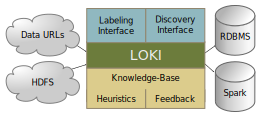
\includegraphics[width=0.8\columnwidth]{graphics/system.pdf}
\caption{System Overview}
\label{fig:overview}
\end{figure}

The overall goal of \systemname is to streamline the process of developing schemas for existing unlabeled or poorly labeled data sets.  
As illustrated in Figure~\ref{fig:overview}, \systemname lives alongside an existing RDBMS or Spark deployment, and takes as input tabular data in the form of a URL or HDFS file path.
\systemname provides users with two modes of interaction: (1) A \emph{labeling} interface that assists users in assigning names to existing columns of data, and (2) A \emph{discovery} interface that helps users to search for columns representing particular concepts of interest.  
Both interfaces are supported by a knowledge-base that combines expert-provided heuristics, learned characteristics, as well as historical feedback gathered from users about already-loaded datasets.
Once the user has labeled or discovered a sufficient set of columns, \systemname generates appropriate data loading/initialization code (e.g., a \texttt{CREATE TABLE} or Spark DataFrame initializer).  


\subsection{Labeling and Discovery}

\begin{itemize}
  \item Declare notation: Set of columns, Rule for column labeling, etc...
  \item Express the labeling problem in terms of this
  \item Express the discovery problem in terms of this
\end{itemize}


\subsection{Approximate Matching Rules}

Outline approximate matching rules: Expert heuristics, rules, etc...
\begin{itemize}
  \item How are approximate KB entries encoded?
  \item How do we unify different types of heuristics?
\end{itemize}


\subsection{Exact Matching Rules}

Outline exact matching rules: Data identity, recording/querying feedback.  Merging conflicts.

\begin{itemize}
  \item How is feedback saved in the KB.
  \item What happens in response to conflicting feedback.  
\end{itemize}
